\documentclass[11pt]{article}
\usepackage[margin=1in]{geometry}
\usepackage{amsmath,amssymb,booktabs,graphicx,hyperref,microtype}
\graphicspath{{docs/papers/paper1/figures/}{figures/}}
\usepackage[numbers]{natbib}
\title{Encode, Generate, Review, Validate:\\Explicit Cognitive Modes with Persistent Goal State in a Shared Transformer}
\author{Paper 1 -- Experimental Inception Draft}
\date{\today}
\begin{document}\maketitle
\begin{abstract}
Decoder-only language models use the same causal transformer stack for understanding a request, generating an answer, and implicitly evaluating what has been generated. We study a minimal alternative that preserves a shared transformer body but introduces explicit operating modes and persistent task state. The model first encodes the complete task with bidirectional self-attention, extracts a latent goal representation $Z_G$, generates causally while conditioned on this latched state, re-encodes the completed output in review mode, extracts a realized-output representation $Z_Y$, and validates the candidate by comparing intended and realized state. We define parameter-, data-, and compute-controlled baselines, machine-checkable multi-constraint generators, held-out near-miss validation, causal interventions on $Z_G$ and mode identity, calibration metrics, and immutable run artifacts. An executable CPU-scale scaffold accompanies this inception draft; it validates the protocol but does not yet support empirical claims.
\end{abstract}

\section{Problem Statement}
A decoder-only transformer must encode a task and generate its solution under a causal mask. Even if a prompt is entirely available before answer generation, hidden representations at prompt position $i$ are constrained to $x_{\le i}$. We test whether separating encode, generate, review, and validate improves goal fidelity while retaining a shared neural substrate. The modes are experimental interventions, not claims of unique correspondence to human cognition.

\section{Architecture}
Let
\begin{equation}
H^{(m)}=F_\theta(X,Z,e_m,\mathcal M_m),
\end{equation}
where $e_m$ is a learned mode embedding and $\mathcal M_m$ a mode-specific attention mask. Encode/review use bidirectional masks; generation is causal. The first design keeps $\theta$ shared.

For an input of length $n$, the causal mask permits attention when $j\leq i$, whereas the bidirectional mask permits every non-padding pair $(i,j)$. Mode embeddings remain present when masks are equal, so mask and mode identity can be ablated separately. All reported baseline models instantiate the same token, position, mode, transformer, goal, review, and validator parameters. We report both total and active parameters; inactive heads are retained to make checkpoint shapes and total parameter counts exactly comparable.

\subsection{Encode and Goal Extraction}
\begin{equation}
H_E=F_\theta(X,\varnothing,e_E,\mathcal M_{bi}),\qquad Z_G=Q_G(H_E).
\end{equation}
$Q_G$ operates before vocabulary projection. The executable V0 uses masked mean pooling followed by a learned projection. Subsequent registered variants compare a special goal token, one learned query, then $k\in\{4,8\}$ facet queries. Shared causal/bidirectional mask operation has precedent \citep{dong2019unified}; the question here is its use inside a persistent goal-state cycle.

\subsection{Generation}
\begin{equation}
p(Y\mid X,Z_G)=\prod_{t=1}^{T}p_\theta(y_t\mid y_{<t},X,Z_G,e_G).
\end{equation}
The V0 conditioning is an additive broadcast projection $h'_{0,t}=h_{0,t}+W_ZZ_G$ applied to the generation input stream. Token-level encoded prompt states are passed into the causal generation pass, isolating bidirectional encoding without requiring a separate decoder. The current executable harness also supports a continuous-prefix diagnostic in which $Z_G$ is projected into a small bank of learned latent prefix vectors prepended to the generation context, and a prefix-KV diagnostic in which separate goal-derived key and value memories are exposed at each self-attention layer without becoming query or residual-stream positions. These mechanisms are related to continuous prefix conditioning \citep{li2021prefixtuning}. Lightweight cross-attention remains a registered follow-up. Goal-conditioned residual gating is deferred. The primary condition latches $Z_G$ throughout generation.

The current executable next-iteration harness additionally supports configurable goal reinjection schedules during generation: input-only, early-layer, periodic, all-layer, and late-layer additive reinjection of the same latched latent condition, together with a continuous-prefix alternative that provides goal access through dedicated latent prefix vectors instead of additive state injection. These are diagnostic controls rather than new headline claims. They ask whether persistent goal influence depends mainly on what $Z_G$ contains, on how often the generator can access it across residual depth, or on the form of the conditioning channel itself.

\subsection{Review and Validation}
For completed output $Y$,
\begin{equation}
H_R=F_\theta(Y,Z_G,e_R,\mathcal M_{bi}),\qquad Z_Y=Q_R(H_R).
\end{equation}
Compare final causal state, an extra causal pass, bidirectional $Y$-only review, and bidirectional $(X,Y)$ review. A validator computes
\begin{equation}
(r,\mathbf r_f,\Delta Z)=V_\phi(Z_G,Z_Y),
\end{equation}
with scalar success probability, optional per-facet satisfaction, and discrepancy state. A baseline head uses
\begin{equation}
u=[Z_G;Z_Y;Z_G-Z_Y;Z_G\odot Z_Y],\quad r=\sigma(\mathrm{MLP}(u)).
\end{equation}

\section{Research Questions and Hypotheses}
RQ1: Does bidirectional task encoding help under matched compute? RQ2: Does latched $Z_G$ improve requirement retention, especially for long outputs? RQ3: Does bidirectional review improve error detection beyond causal alternatives? RQ4: Does $(Z_G,Z_Y)$ validation outperform simply rereading prompt and answer? RQ5: Can validation improve selection/retry under compute controls? RQ6: Do modes and $Z$ have identifiable causal/mechanistic effects?

We expect encode gains for distributed/late constraints, $Z$ gains to increase with generation length and simultaneous requirements, review gains for global inconsistencies/omissions, and intended-realized comparison to improve facet localization and candidate ranking.

\section{Controlled Dataset Suite}
\subsection{Multi-Constraint Generation}
Each prompt contains $K$ independently checkable requirements. Vary $K$, prompt length, requirement position, distractor count, output length, and requirement type (content, order, format, exclusion, cross-part consistency). Store structured ground truth and deterministic validators.

\subsection{Late Constraints and Distractors}
Move decisive constraints to the end while holding semantics fixed. Add instruction-like non-authoritative distractors. These tasks test global encoding and whether $Z$ captures task role rather than lexical salience.

\subsection{Ordered and Deterministic Tasks}
Require multiple ordered sections or transformations with independent checks. Include arithmetic, symbolic transformations, structured data, and small code tasks with executable tests.

\subsection{Candidate Pairs}
Construct valid/near-miss pairs differing in exactly one requirement for facet validation, ranking, and mechanistic probes.

\subsection{Executable V0 Generator}
The V0 generator represents each requirement as a separately checkable binary facet while varying facet count, order, filler length, and the number of explicitly delimited distractors. One authoritative requirement is always placed last. Train, validation, and test use both disjoint deterministic example namespaces and different prompt topologies: grouped requirements, reversed/grouped requirements, and locally interleaved authoritative/distractor blocks. The ordered target contains one token per active facet. Training corruptions flip one facet, validation targets the late facet, and test corruptions mix single and double flips, truncation, and invalid end markers. A counterfactual prompt and target flip the same authoritative facet, enabling a directed $Z_G$ substitution test. A selectable canonical-goal diagnostic supplies the encoder only the authoritative requirement blocks in canonical order, with a reversed-order paraphrase, while leaving the generator's held-out content channel unchanged. This isolates latent channel capacity from goal parsing under distractors. Every run records the generator version, split family, goal-prompt style, and SHA-256 hash of all materialized full, generation, goal, paraphrase, counterfactual, target, and corruption channels. This synthetic vocabulary tests the architecture and harness, not general language understanding; natural templates, executable transformations, code tasks, and pretrained backbones are required in the next empirical stage.

\section{Baselines and Ablations}
\begin{center}\begin{tabular}{lll}\toprule
ID & Encode/State & Review/Validation\\\midrule
B0 & causal decoder, no $Z$ & none\\
B1 & B0 + matched residual MLP & none\\
B2 & extra causal encode, no $Z$ & none\\
B3 & bidirectional encode, no $Z$ & none\\
B4 & causal encode + $Z_G$ & none\\
B5 & bidirectional encode + $Z_G$ & none\\
B6 & B5 & final generation state\\
B7 & B5 & extra causal review\\
B8 & B5 & bidirectional $Y$ review\\
B9 & no persistent $Z_G$ & bidirectional $(X,Y)$ reread\\
B10 & bidirectional encode + $Z_G$ & bidirectional $(X,Y)$, $(Z_G,Z_Y)$\\
\bottomrule\end{tabular}\end{center}
All rows have the same instantiated parameter count. B1 activates a capacity-matching residual MLP without task state; B2 spends an extra causal pass; B3 and B5 pass token-level encoded prompt states into generation. Later work compares shared weights with small mode adapters and fully separate modules only if bidirectional/causal interference is observed.

\section{Training}
The executable training protocol supports an initial goal warmup followed by joint generation, goal decoding, validation, facet localization, and pairwise ranking. Warmup minimizes masked facet reconstruction and same-goal paraphrase invariance before $Z_G$ is used as a generation condition. Joint checkpoints are selected only by loss on the held-out validation topology, with configurable evaluation cadence and bounded early stopping. The broader empirical progression remains: Stage 0 establishes a base LM or small pretrained model with exact disabled-feature parity. Stage 1 mixes causal/bidirectional mask training with explicit mode embeddings. Stage 2 adds goal objectives:
\begin{equation}
L=L_{LM}+\lambda_G L_G,
\end{equation}
where $L_G$ may include facet decoding, paraphrase-invariant contrastive learning, structured requirement reconstruction, or predictive usefulness. Stage 3 adds
\begin{equation}
L=L_{LM}+\lambda_G L_G+\lambda_V L_V+\lambda_R L_{rank}.
\end{equation}
Use deterministic external labels where possible. Only after calibration should Stage 4 test retry/revision or limited RL.

For V0, $L_G$ combines masked binary facet decoding with cosine paraphrase invariance, $L_V$ is BCE on valid and deterministically corrupted candidates, and $L_{rank}=\log(1+\exp(r^- - r^+))$. A separate multilabel BCE trains facet satisfaction. Loss weights, warmup duration, optimizer, seed, validation cadence, and gradient clipping are configuration values rather than hidden constants.

\section{Inference Policies}
Single generation is the base. Validation-only scores without changing output. Best-of-$N$ selects $Y^*=\arg\max_i r_i$. Threshold retry regenerates if $r<\tau$. Revision conditions on discrepancy:
\begin{equation}
Y'=G(X,Z_G,Y,\Delta Z).
\end{equation}
Every result reports model calls, generated tokens, approximate FLOPs, latency, and wall time.

\section{Metrics}
\textbf{External task metrics:} accuracy, exact match, F1, full-task pass rate, fraction of satisfied constraints, per-facet recall, executable-test pass rate, and degradation with generation length.

\textbf{Validation:} AUROC, AUPRC, Brier score, expected calibration error, ranking accuracy, best-of-$N$ oracle gap, false-positive rate on confidently wrong outputs, and facet localization accuracy.

\textbf{Goal representation:} same-goal paraphrase similarity, different-goal separation, linear-probe facet recovery, $Z$ stability, sensitivity to requirement position, and causal interventions.

\textbf{Mechanistic:} attention entropy/dilution; residual update norms; update/state alignment; refinement versus complementary/orthogonal update versus interference; layer/head similarity; mode-conditioned representation similarity; temporal feature stability.

\section{Causal Intervention Suite}
The executable evaluation zeroes $Z_G$; shuffles it across examples; substitutes a same-goal paraphrase state; substitutes a state from a prompt with one flipped facet; removes mode embeddings while retaining masks; and swaps encode/generate embeddings. Exact-match interventions use the same active-facet and required-end-token criterion as primary evaluation. Counterfactual evaluation separately reports whether the targeted facet changes, whether it changes while all untouched active facets remain correct, and whether the complete counterfactual target is exact; raw intervention generations are retained for audit. Registered extensions perturb learned facet directions, freeze/unfreeze $Q_G$, swap review identity, and compare latched with recomputed $Z_G$. A genuine goal representation should preserve behavior under same-goal substitution, degrade under zero/shuffle interventions, and alter the targeted output facet under counterfactual substitution. Correlation or probe accuracy alone is insufficient.

\section{Compute and Parameter Controls}
Mode architectures can win trivially by spending extra compute. Report training/inference FLOPs, forward-pass count, sequence lengths, parameter count, and latency. Compare review against equivalent causal compute; best-of-$N$ validation against random and likelihood-based selection; and $Z$ parameters against matched width/MLP additions. Distinguish quality-per-sample from quality-per-compute.

The harness counts actual shared-transformer calls and non-padding token positions at runtime. It reports base generation, validation, selection-time validation, and diagnostic interventions separately, together with instantiated and active parameter counts. The implementation-level estimate is $2P$ FLOPs per forward token-position and $6P$ per training token-position for $P$ parameters; this coarse proxy is always accompanied by measured wall time and raw counts. It is not used as a substitute for profiler-based FLOPs in headline experiments. Prompt encoding and $Z_G$ are computed once, cached, and latched for an autoregressive candidate; unit tests assert one encode call plus one causal call per generated token.

\section{Expected Failure Modes}
\textbf{Shortcut validation:} mitigate with held-out generators and adversarial near-misses.\\
\textbf{Goal collapse:} $Z$ may encode prompt identity rather than intent; test paraphrases, probes, and substitutions.\\
\textbf{Mode collapse:} embeddings may be ignored; probe and swap modes.\\
\textbf{Bidirectional/causal interference:} shared weights may lose generation quality; only then test adapters/partial sharing.\\
\textbf{Self-confirmation:} generator and validator may share blind spots; use deterministic external validators.\\
\textbf{Compute illusion:} gains may vanish under matched budget; treat this as a valid negative result.

\section{Future Goal Dynamics}
If $Z_G$ reliably represents explicit tasks and $\Delta Z$ unmet requirements, next introduce explicit task transitions and completion evidence. Future state can distinguish root, active, parent, pending, blocked, suspended, and completed goals. Only after known hierarchies work should the model learn decomposition
\begin{equation}
D(z_g,h)\rightarrow\{z_{g_1},\ldots,z_{g_k}\}.
\end{equation}
Thus Paper 1 is a substrate for planning rather than an attempt to solve planning.

\section{Future Gated Residual Integration}
Once $Z$ is meaningful, test
\begin{equation}
h_{\ell+1}=h_\ell+g_\ell(h_\ell,Z,m)F_\ell(h_\ell),
\end{equation}
asking whether explicit goals determine which computations should be active. This is intentionally not required by Paper 1.

\section{Future PRA and Progressive Tool Integration}
PRA addresses selective memory; this paper addresses goal/state control. Later typed references may represent tasks, tools, skills, documents, and observations, with progressive materialization conditioned on the active goal. Tool selection can then become goal-conditioned affordance/action selection rather than repeated schema-token processing. These are integration targets, not dependencies.

\section{Feedback, RL, and Consolidation}
A deployed system can accumulate tuples $(X,Z_G,Y,Z_Y,r,feedback)$ plus deterministic tests, retries, accepted edits, tool outcomes, and controller choices. This is richer experience than plain next-token text. Online base-weight learning is deferred. Later sleep/consolidation should use provenance-aware replay, adapter-only candidate updates, held-out regression gates, and rollback. RL should reward externally grounded transitions rather than blindly maximize the model's own validator.

\section{Relation to Prior Work}
Unified language models demonstrate shared weights under bidirectional and causal masks \citep{dong2019unified}; encoder-decoder transformers separate encoding from decoding \citep{vaswani2017attention,raffel2020exploring}; continuous prefixes condition generation on learned latent vectors \citep{li2021prefixtuning}; self-consistency uses multiple reasoning samples \citep{wang2023selfconsistency}; and verifiers or reward models explicitly score outputs \citep{cobbe2021verifiers,ouyang2022training}. The present work asks whether persistent intended task state, explicit modes, and a realized-output representation provide value beyond these components under controlled composition.

\section{Success Criteria}
A strong result requires more than benchmark improvement. Across multiple seeds and held-out task generators, at least several of the following should hold: bidirectional encode improves constraint fidelity under compute control; $Z$ improves long-output retention; interventions on $Z$ predictably alter goal satisfaction; review improves externally verified error detection; validator scores are calibrated and generalize; validation improves selection/retry at competitive compute; and internal metrics show interpretable mode/goal effects.

A strong negative result is also informative: if the causal decoder reproduces all benefits under matched resources, explicit modes or $Z$ should not be retained merely for conceptual appeal.

\section{Reproducibility Plan}
Every run stores git commit, complete config, seed, dataset generator/version/hash, architecture and parameter count, optimizer/schedule, hardware, training/evaluation time, token/forward-pass counts, raw predictions, validator outputs, and plot/table source data. Headline results use multiple seeds. Raw run outputs are immutable.

The repository exposes CPU smoke and overfit gates, one-seed unstaged and staged held-out pilots, a main configuration, and a five-seed baseline suite. A timestamped run directory is created with exclusive semantics and contains the resolved configuration, provenance, materialized dataset hashes, epoch history, checkpoint, reload verification, raw JSONL predictions, and scalar metrics. Timestamped suite summaries include confidence intervals and seed-paired differences. Unit tests check generator determinism, split-family separation, multiple corruption types, counterfactual integrity, dataset-hash stability, exact parameter matching, active parameter accounting, causal prefix invariance, bidirectional suffix sensitivity, cached-encode call counts, seeded optimizer determinism, and finite multi-objective losses. Smoke and memorization-gate completion establish only that the protocol executes and can fit data; neither is entered into headline result tables.

\section{Implementation Diagnostic (Not a Headline Result)}
Before launching a multi-seed study, we ran a seed-0 optimization diagnostic with a small Transformer trained from scratch. A shared-example memorization gate reached 1.0 exact match for B0, B5, and B10 after 100, 250, and 250 optimizer updates, respectively; B10 also reached 1.0 validator AUROC. Thus the representative paths can fit the task and validator when generalization is deliberately removed. Table~\ref{tab:pilot-diagnostic} instead uses disjoint example namespaces, held-out prompt topologies, and held-out corruption families. ``Staged'' adds 15 goal-warmup epochs and validation-selected joint training. Effects are the decrease in exact match caused by the intervention; positive values indicate degradation.

\begin{table}[ht]
\centering
\begin{tabular}{llrrrrr}\toprule
Protocol & Baseline & Exact & Facet & Zero $Z_G$ & Shuffle $Z_G$ & Val. AUROC\\\midrule
Unstaged & B0  & .430 & .797 & ---   & ---    & ---\\
Unstaged & B5  & .109 & .553 & .020  & .000   & ---\\
Unstaged & B10 & .102 & .539 & -.004 & .000   & .476\\
Staged   & B5  & .168 & .604 & .090  & .004   & ---\\
Staged   & B10 & .156 & .601 & .031  & -.016  & .575\\\bottomrule
\end{tabular}
\caption{Seed-0 implementation diagnostic on the held-out V0 generator. This table is not a hypothesis test.}
\label{tab:pilot-diagnostic}
\end{table}

The held-out result is presently negative. Staging improves B5 and B10 relative to their unstaged variants, but both remain far below causal B0. Zeroing $Z_G$ becomes harmful, yet shuffling it does not consistently reduce accuracy, which indicates a generic conditioning effect rather than reliable example-specific control. B10 validation rises above chance (AUROC .575; pairwise ranking accuracy .637) but is not strong enough for selection claims. These observations block a costly multi-seed headline run: the next iteration should strengthen example-specific goal conditioning and the held-out validator objective, then require shuffle and counterfactual interventions to pass preregistered gates. The exact source values and interpretation are stored in \texttt{results/pilot\_iteration2.json}.

\section{Persistent Goal State as a Causal Channel}
The current pilot supports a narrower claim than the original aspiration. The model can be sensitive to the presence or ablation of $Z_G$, but this alone does not show that $Z_G$ is an example-specific goal representation. In particular, a latent can influence generation while still acting as a generic auxiliary bias, a compressed prompt statistic, or a training-dependent shortcut. We therefore adopt a stricter operational criterion:
\begin{quote}
A latent state represents the goal to the extent that interventions on that state, while holding relevant non-goal content fixed, cause predictable goal-consistent changes in behavior.
\end{quote}

The next iteration therefore begins by forcing $Z_G$ to become the only goal-information channel. Tasks are split into content $C$ and goal specification $G$, the generator receives $C$ directly, and the requested behavior must be conveyed through $Z_G=\mathrm{Encode}(G)$. The primary controls are correct-$Z$, shuffled-$Z$, zero-$Z$, constant-$Z$, and random-$Z$ generation. A causal gate is passed only if correct-$Z$ materially outperforms shuffled-$Z$ on held-out synthetic tasks. Held-out probes on frozen $Z_G$ then separate goal decodability from goal use: high probe accuracy with weak shuffle sensitivity indicates that encoding works but conditioning fails, whereas low probe accuracy indicates that the representation itself is inadequate.

This stricter framing also motivates a refined persistence hypothesis. Persistent goal state may provide little or no benefit for short generations or shallow networks, yet become increasingly useful when intent must remain influential across many autoregressive steps or many residual transformations. The relevant signatures are therefore not limited to aggregate exact match. We will first test whether richer latent capacity and repeated per-layer access to the same latent improve correct-versus-shuffled $Z_G$ effects in the Z-only setting, then ask whether those effects grow with generation horizon, grow with depth, or reduce late-output drift under long-horizon constraints. Negative outcomes remain informative: if $Z_G$ stays weak even when direct goal tokens are removed, then the current representation or conditioning mechanism should be revised before larger benchmark runs.

As of Sunday, August 23, 2026, the reinjection and conditioning diagnostics show a more specific pattern than the initial negative result. Under the same small held-out Z-only strong-goal setting, naive all-layer additive reinjection of a single-vector $Z_G$ performs worse than the input-only condition: exact match falls from .148 to .119, facet satisfaction falls from .608 to .526, the shuffled-goal effect falls from .041 to .027, and the zero-goal effect falls from .059 to .051. A periodic reinjection schedule that reintroduces the same latent every two layers partially recovers some of this loss, but still does not surpass the input-only baseline: exact match rises only to .121, facet satisfaction to .554, and the shuffled-goal effect to .031, while the zero-goal effect drops further to .020. By contrast, late-layer reinjection is the first reinjection schedule that improves on the input-only baseline: exact match rises to .164, facet satisfaction to .619, the shuffled-goal effect to .055, and counterfactual facet substitution success to .951. However, combining the two individually promising modifications---multi-vector goal state and late-layer reinjection---is sharply negative in this first pilot: exact match falls to .057, facet satisfaction to .446, the shuffled-goal effect nearly disappears at .002, and counterfactual facet substitution success drops to .746. The first non-additive conditioning diagnostic, continuous prefix conditioning with four learned latent prefix tokens, is competitive with the best additive late-layer schedule rather than clearly superior or inferior: exact match reaches .162, facet satisfaction .624, the shuffled-goal effect .057, and counterfactual facet substitution success .889. A same-day prefix-length sweep then shows that the result is not a one-setting anomaly but also not monotonic with prefix size: two prefix tokens yield exact match .156, facet satisfaction .615, and the strongest shuffled-goal effect at .063; four tokens yield exact match .162 and the strongest facet satisfaction at .624; eight tokens keep exact match at .162 but degrade facet satisfaction to .593 and reduce held-out linear-probe facet accuracy from roughly .656/.645 to .601. The two-memory prefix-KV diagnostic reaches .143 exact match, .609 facet satisfaction, and a .049 shuffled-goal effect, below both the matched two-token continuous prefix and the best late-layer additive condition despite its additional layerwise K/V parameters. The initially matched eight-epoch direct text-prefix control reaches only .102 exact match and .518 facet satisfaction, but its validation LM loss remains 1.271, revealing severe under-optimization. A 40-epoch convergence follow-up with the same direct architecture reaches .975 exact match and .995 facet satisfaction, with validation LM loss .021. Thus the apparent short-run latent advantage is an optimization-speed artifact, not evidence that latent conditioning outperforms ordinary goal tokens; the direct causal route is decisively stronger once trained to convergence in this pilot. Among latent mechanisms only, the evidence favors selective late access or a short continuous prefix over naive repeated additive access, richer latent combinations, or prefix-KV. The strongest Z-only mechanism must now receive a comparable convergence run before causal gates are judged, and prefix-KV should not be carried into larger sweeps unless depth-specific evidence later motivates revisiting it. Exact source values are stored in \texttt{results/text\_prefix\_convergence\_pilot\_iteration1.json}, \texttt{results/z\_only\_prefix\_kv\_pilot\_iteration1.json}, and the preceding context, reinjection, and prefix summaries.

The converged single-vector late-layer Z condition improves to .197 exact match and .642 facet satisfaction. Under the corrected end-token-aware intervention metric, shuffling reduces exact match to .096, a .102 absolute causal effect, while zeroing reduces it to .080. Longer training therefore strengthens example-specific use of $Z_G$, but it does not pass the preregistered gates: held-out linear-probe facet accuracy is only .661 despite .918 on training goals, and although the substituted target facet changes correctly in .936 of cases, only .285 preserve every untouched active facet and satisfy the complete counterfactual target. The direct causal baseline remains far stronger at .975 exact match. We therefore do not yet restore direct goal access or launch depth/time grids. The next diagnostic isolates channel capacity and conditioning use with a canonical authoritative goal prompt before reintroducing distractors and held-out goal topology. Exact values and the gate decision are stored in \texttt{results/z\_only\_convergence\_pilot\_iteration1.json}.

That canonical-goal diagnostic sharply localizes the failure. With the same single-vector late-layer conditioning, task exact match and facet satisfaction both reach 1.0. Linear and MLP probes recover every held-out facet and achieve 1.0 joint exact match. Shuffling $Z_G$ reduces exact match to .100, a .900 causal effect; zero, constant, and random interventions produce comparably large degradation. Replacing one goal facet yields 1.0 targeted, isolated, and complete counterfactual success, while a reversed-order same-goal substitution retains .988 exact match. Gates 1--3 therefore pass at one-seed diagnostic scale when the encoder receives only authoritative canonical requirements. The result establishes functional sufficiency of the single-vector latent channel and late-layer conditioning, but not superiority over direct text: canonical goal construction supplies privileged semantic extraction. The earlier rendered-goal failure is primarily a goal-extraction and held-out-topology problem. We may now run a one-seed canonical direct-exposure curve, while deferring headline claims and the full depth--time grid until replication and a persistence gate. Exact values are stored in \texttt{results/z\_only\_canonical\_goal\_pilot\_iteration1.json}.

For the direct-exposure curve, $p_{\mathrm{direct}}\in\{0,.25,.5,.75,1\}$ controls deterministic probabilistic insertion of authoritative canonical requirement blocks into the generator's ordinary-token prefix while keeping the encoded $Z_G$ channel active. Separate matched models are trained at each exposure level. Within each condition we measure $D_Z(p)=\mathrm{Score}(Z_{\mathrm{correct}},p)-\mathrm{Score}(Z_{\mathrm{shuffled}},p)$. A decreasing curve would indicate that the generator bypasses persistent latent state as direct symbolic access becomes available; independently trained exposure conditions also permit adaptation, so any trend will be treated as a behavioral route-preference diagnostic rather than a pure inference-time intervention.

Figure~\ref{fig:z-necessity} shows that the expected smooth bypass signature does not appear. Correct-Z exact match remains 1.0 throughout, while $D_Z$ under exact match stays between .873 and .902 from no direct access through complete direct access. The facet-level effect similarly stays near .497 through $p=.75$ and declines only to .433 at $p=1$. At the complete-direct endpoint, zero-Z facet satisfaction rises to .738, confirming that direct goal tokens are usable when latent conditioning is absent. Nevertheless, counterfactual $Z_G$ still produces the complete latent-consistent output in .926 of cases despite conflicting direct requirements. In this shallow independently trained setting, late-layer additive $Z_G$ is therefore a dominant route rather than a channel the model bypasses. This is an architectural route-preference diagnostic, not evidence that latent access improves over direct-only text.

\begin{figure}[t]
\centering
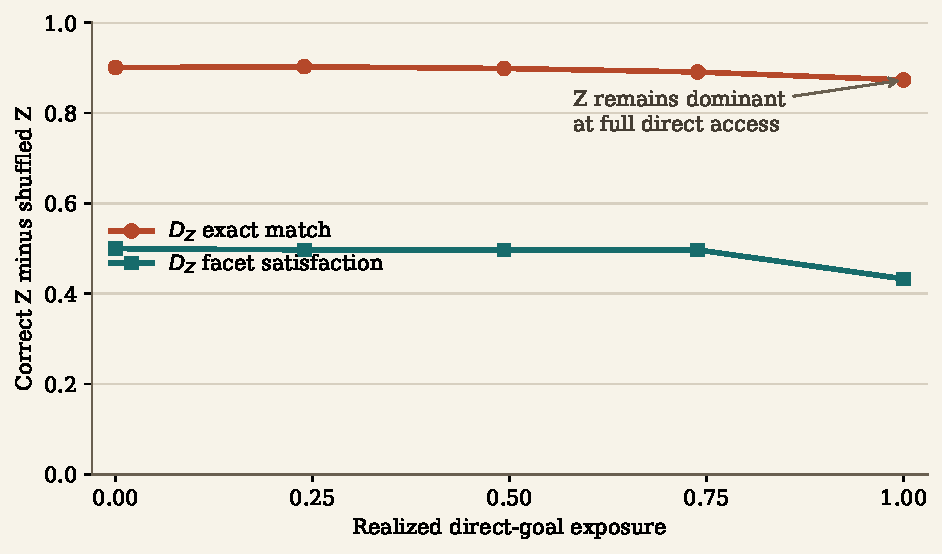
\includegraphics[width=.72\linewidth]{figures/z_necessity_curve.pdf}
\caption{Canonical direct-goal exposure curve. The exact-match and facet-satisfaction effects of shuffling $Z_G$ remain large even as direct symbolic exposure increases. Source: \texttt{results/z\_necessity\_curve\_pilot\_iteration1.csv}.}
\label{fig:z-necessity}
\end{figure}

\subsection{Scheduled Generation-Horizon Diagnostic}

The temporal-persistence task does not pad or repeat meaningless prose. Its content channel provides a long sequence of varying facet requests; each target position must emit the value of the requested facet under the original six-facet goal. Every six-position block uses a new deterministic permutation, preventing a fixed repeated output block from satisfying the task. The first matched point uses five blocks, yielding 31 output tokens including the end marker. Evaluation reports aggregate exact match and satisfaction, satisfaction in four equal output-position quartiles, and early-minus-late goal drift for both conditions; corresponding shuffled-$Z_G$ quantities are additionally reported only for the latent condition. Canonical late-layer Z is compared with a direct-only causal prompt. Both instantiate the same 1,152-position model so later target horizons remain parameter-matched.

The first one-seed point is an optimization diagnostic rather than a persistence result. Direct goal tokens reach .637 per-position satisfaction, compared with .170 for correct $Z_G$ and .090 for shuffled $Z_G$; the resulting .080 correct-minus-shuffled effect confirms modest example-specific Z use, but direct text remains .467 better overall. Direct satisfaction declines from .764 in the first output quartile to .483 in the fourth, exposing position-dependent degradation. Correct-Z satisfaction changes only from .187 to .167, but this small .019 drift occurs near floor and cannot count as successful persistence. Sequence exact match is zero for both conditions. Moreover, the direct run selects epoch 40 of 40 and the Z run epoch 39 of 40 while their validation language-model losses remain .621 and 1.209, respectively, so neither supplies a converged matched comparison. We therefore stop the horizon sweep at this gate and first extend optimization of the 31-token point to an 80-epoch ceiling with patience of eight validations, changing no data, architecture, optimizer, or evaluation setting. Exact values are stored in \texttt{results/horizon\_32\_pilot\_iteration1.json}.

The extended-budget comparison resolves the task-level ambiguity but not in favor of Z. The direct condition reaches 1.0 exact match and 1.0 satisfaction in every quartile, proving that the varying 31-token schedule is learnable and that its pilot drift was an optimization artifact. Under the identical 80-epoch ceiling, correct-Z satisfaction reaches only .176 and exact match remains zero, a negligible .005 satisfaction gain over the 40-epoch pilot. Shuffled-Z satisfaction is .090, so the .086 causal effect still demonstrates example-specific latent use; however, use of Z is not sufficient for reliable scheduled retrieval. Correct-Z satisfaction declines from .214 to .156 across quartiles, while direct text has zero drift at ceiling. This strongly suggests that one globally added vector does not provide the same query-dependent access to six facet values as direct goal tokens. We therefore keep longer horizons gated and next compare structured latent access at the same 31-token point. The first such control keeps the single-vector encoder fixed but projects Z into six continuous prefix tokens available to attention at every layer, isolating addressable presentation from increased encoder-state capacity. Exact values are stored in \texttt{results/horizon\_32\_extended\_optimization\_iteration1.json}.

The six-token continuous-prefix control does not repair the deficit. It reaches .172 satisfaction and zero exact match, compared with .176 and zero for matched late-layer additive Z. Its correct-minus-shuffled satisfaction effect rises slightly from .086 to .093, confirming latent use, but the .007 early-to-late change again occurs near floor. This negative result is especially informative because the prefix condition exposes more active conditioning parameters and makes six memory positions attention-addressable at every layer while preserving the same one-vector encoder. Presentation alone is therefore insufficient. The next 31-token isolation holds that six-token interface fixed while replacing the pooled vector with six learned-query encoded vectors, testing encoded-state structure separately from presentation. These learned vectors are not presumed facet-aligned; that stronger interpretation requires swaps and probes. Exact values are stored in \texttt{results/horizon\_32\_structured\_prefix\_iteration1.json}.

Generic multi-vector encoding also fails the behavioral gate. Six learned-query goal vectors with the same six-token prefix reach .185 satisfaction and zero exact match, only .013 above the one-vector prefix despite increasing corrected active parameters from 205,830 to 331,014. Yet held-out validation goal loss falls from .0726 to .00329, showing that the larger state supports the auxiliary facet objective. The correct-minus-shuffled satisfaction effect remains essentially unchanged at .093. This creates a sharp decodability--use separation: raw encoded capacity improves, but the generator still cannot reliably select the required facet value from latent memory. Adding more unspecialized vectors is therefore not justified. The active counts correct an instrumentation error that included unexecuted conditioning projections and omitted direct query parameters; total parameter counts and behavioral metrics are unaffected, while raw artifacts retain originally reported values and total-parameter-based approximate FLOPs. Future FLOP estimates use executed-mode active counts. The next isolation explicitly maps each canonical requirement token to its known facet slot, supervises each slot's value through a shared head, and exposes the six slots directly as latent prefix memory without flattening or remixing them. A matched counterfactual replaces one slot and measures selected-facet change, untouched-facet preservation, and full exact match. Exact preceding values are stored in \texttt{results/horizon\_32\_multivector\_prefix\_iteration1.json}.

The aligned-slot diagnostic is also negative. It reaches .161 satisfaction and zero exact match, below the generic six-vector prefix condition, while correct-minus-shuffled satisfaction is .081. The stronger localized intervention fails sharply: replacing the selected facet slot with its matched counterfactual changes the five corresponding scheduled positions correctly only .008 of the time, preserves untouched positions at only .187 satisfaction, and never produces a complete counterfactual sequence. Thus explicit slot extraction, slot-level value supervision, and direct slot presentation do not establish localized behavioral control. Because direct text solves the same schedule perfectly, task learnability is no longer a viable explanation. Longer horizons and facet-swap claims remain gated. The next interface control adds learned facet-slot identity and generation-prefix position embeddings, two signals ordinary generation tokens carry but the failed direct slots omitted; the unsignaled condition remains unchanged for reproducibility. Another failure would motivate an encode--generate gradient-compatibility diagnostic rather than further capacity. Exact values are stored in \texttt{results/horizon\_32\_facet\_slot\_prefix\_iteration1.json}.

That narrow signaling repair produces the first large long-schedule Z improvement. Adding slot identity and generation-prefix position raises correct-Z satisfaction from .161 to .743 and the correct-minus-shuffled effect from .081 to .369. The matched slot intervention also becomes substantially localized: selected-facet positions reach .513 satisfaction and untouched positions .738, compared with .008 and .187 without signals. This establishes that latent prefix states require token-like identity and position cues to become usable; compression or slot supervision alone was not the dominant missing ingredient. The result is nevertheless incomplete: task and counterfactual exact match remain zero, epoch 80 is selected, and validation language-model loss is still declining at .308. We therefore extend this exact 31-token condition to a 120-epoch ceiling with patience of ten validations, changing no seed, data, model, optimizer, slot interface, or causal evaluator, before increasing horizon or claiming complete facet-level control. Exact values are stored in \path{results/horizon_32_facet_slot_signaled_iteration1.json}.

The convergence extension passes the 31-token task and causal gates. Correct Z reaches 1.0 exact match and satisfaction in every output quartile, while shuffled Z falls to .0156 exact match and .503 satisfaction, yielding correct-minus-shuffled effects of .984 and .497. Replacing one facet slot produces the complete counterfactual sequence in .672 of examples and preserves untouched positions at .998 satisfaction; selected-facet positions reach .703. Thus the compact latent channel supports perfect scheduled generation and strong localized control once it has explicit slot identity, generation position, and sufficient optimization. Localized control is not yet perfect, and epoch 120 remains selected despite validation language-model loss reaching .0068, so this remains a one-seed mechanism diagnostic. It justifies the next approximately 64-token point with matched direct and shuffled controls, not the full grid or headline replication. That point uses ten independently shuffled six-facet blocks, yielding 61 output tokens including the end marker, while preserving the seed, architecture, data sizes, optimizer, 120-epoch ceiling, and causal evaluator. The direct-text gate does not converge within that ceiling: exact match is zero, facet satisfaction is .678, and validation loss is still falling rapidly at the selected final epoch (.473). We therefore classify 61-token learnability as unresolved, extend direct-text optimization with all other factors fixed, and defer the matched Z run. Exact values are stored in \path{results/horizon_64_direct_iteration1.json}; exact 31-token values remain in \path{results/horizon_32_facet_slot_signaled_convergence_iteration1.json}.

\begin{figure}[t]
\centering
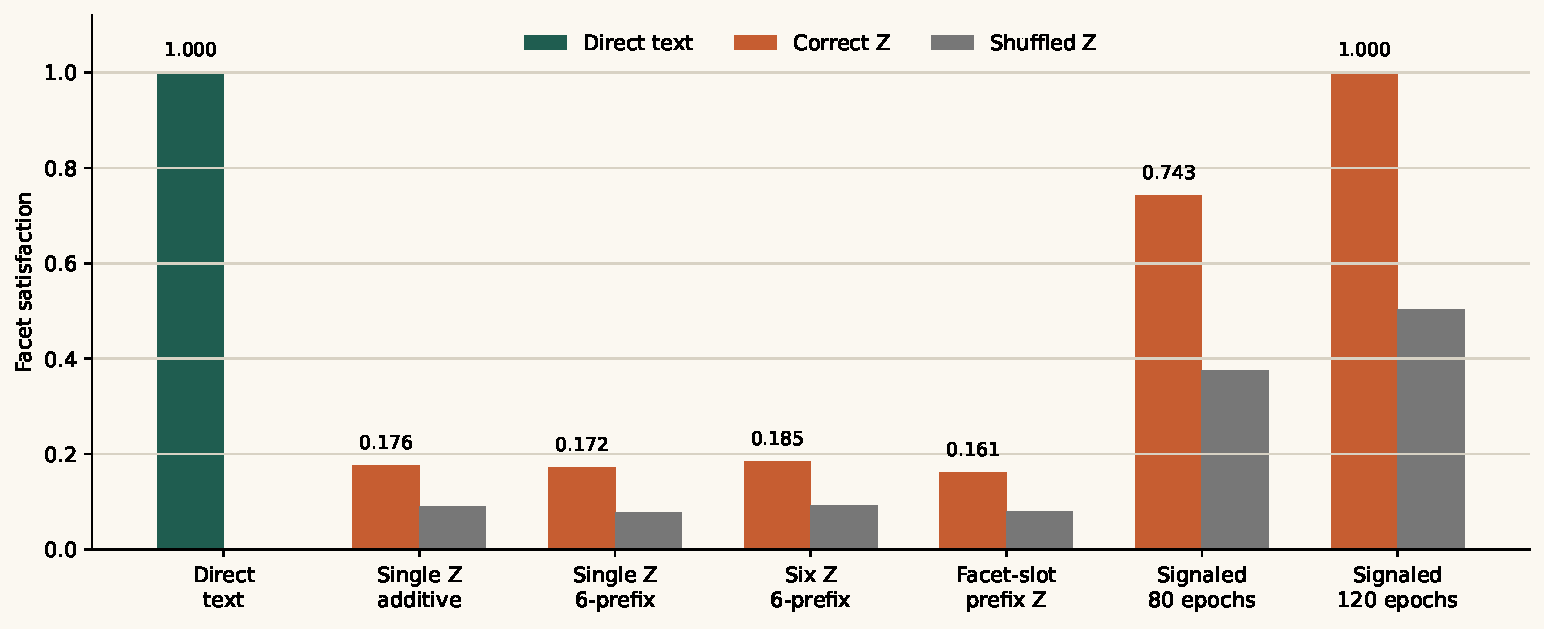
\includegraphics[width=.76\linewidth]{figures/horizon_32_conditioning_comparison.pdf}
\caption{Matched 31-token conditioning comparison. Explicit identity and position signals sharply improve facet-slot Z; with extended optimization it reaches the direct-text ceiling while preserving a large correct-versus-shuffled gap. Source: \texttt{results/horizon\_32\_conditioning\_comparison\_iteration1.csv}.}
\label{fig:horizon-conditioning}
\end{figure}

\begin{figure}[t]
\centering
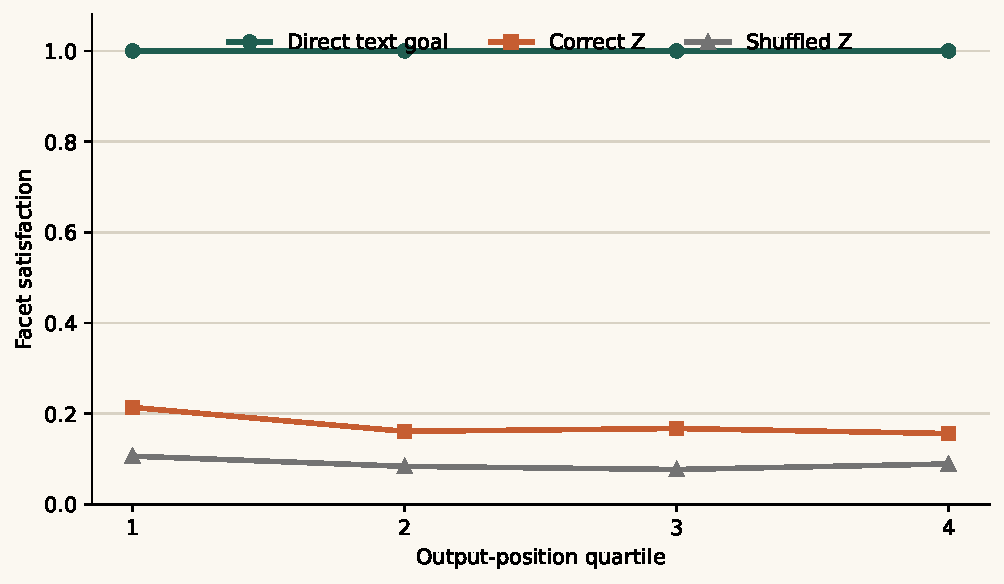
\includegraphics[width=.72\linewidth]{figures/horizon_32_extended_quartiles.pdf}
\caption{Facet satisfaction after the extended matched budget. Direct goal access reaches ceiling in every output quartile; correct $Z_G$ remains low but above shuffled $Z_G$. Source: \texttt{results/horizon\_32\_extended\_optimization\_iteration1.csv}.}
\label{fig:horizon-32}
\end{figure}

\section{Conclusion}
Encode--Generate--Review--Validate is intended as the smallest rigorous test of a broader idea: functions currently forced into homogeneous autoregressive computation may benefit from explicit mode and persistent task state. The design preserves shared weights to avoid explaining gains through parameter multiplication, uses external validation to avoid circular self-evaluation, and emphasizes causal/mechanistic analysis. If successful, it creates a controlled bridge from next-token models toward multi-timescale goal dynamics, selective computation, progressive memory, tools, and reinforcement learning. If unsuccessful, its ablations identify which proposed cognitive distinctions are unnecessary.

\bibliographystyle{plainnat}\bibliography{../common/references}
\end{document}
